
\chapter{绪论}

\section{研究背景}

\indent 流体仿真作为一种重要的物理模拟技术,能够通过计算流体力学和数值计算方法,模拟水、烟雾、火焰等自然现象的动态行为,被广泛应用于科学计算、工程设计、影视制作、游戏开发、虚拟现实(VR)等领域。通过流体仿真,研究者和开发者可以直观地呈现复杂的自然过程,以满足逼真的视觉体验或精确的工程需求。传统的流体仿真通常依赖于复杂的计算模型,尤其在追求高精度和大规模仿真效果的场景中,流体仿真往往需要借助高性能计算平台,如 PC、工作站甚至是 GPU 集群\cite{kipfer2004uberflow},才能满足实时模拟的需求。
\newline
\indent 随着移动设备(如智能手机和平板电脑)硬件性能的提升,用户对高质量图形和物理仿真效果的需求日益增长。流体仿真作为一种复杂的物理模拟方法,具有广泛的应用前景。然而,移动设备在功耗、性能和内存带宽等方面的限制,使得在移动端实现高效且低功耗的3D流体渲染面临诸多挑战。一方面,流体渲染需要模拟复杂的物理现象,如流动、反射、折射和透明度变化,这些计算任务对硬件资源的消耗巨大;另一方面,移动设备的续航能力和散热性能有限,这要求我们在实现逼真视觉效果的同时,必须兼顾功耗控制和性能优化。
\newline
\indent 针对实时仿真需求,近年来研究者们对传统的流体仿真算法进行了多种轻量化改造。光滑粒子流体动力学(SPH)算法\cite{muller2003particle}作为一种常用的流体仿真算法,广泛应用于模拟水流等粒子流体,但计算复杂度较高。 Viccione\cite{viccione2008defining}等人通常通过简化邻域搜索等方法优化 SPH 算法,以减少其计算量和内存消耗。另一种常用的流体仿真方法是位置约束动力学(PBF)\cite{macklin2013position},由于其对于约束条件的处理较为高效,适合低精度、轻量化的实时仿真应用。PBF 算法通过减少约束计算复杂度和优化求解流程,使其在保证仿真效果的同时降低了资源占用。除了计算优化之外,渲染方法的简化也是流体仿真轻量化的重要一环,研究者们通过简化着色器设计、减少光照计算\cite{kunimatsu2001fast}等,来降低流体仿真渲染的资源消耗。近期 Zhang\cite{zhang2024real}等人的工作利用屏幕空间渲染的 SPH 实现了多相流流体的实时渲染。而随着机器学习技术的发展,一些工作将深度学习应用于流体仿真\cite{brunton2020machine},Brunton\cite{pack2018toward}等人将机器学习与 FLIP 流体模拟方法相结合,得到了实时模拟的效果。
\newline
\indent 尽管上述方法在轻量化流体仿真方面取得了一定进展,但当前流体仿真技术仍难以在移动设备上实现实时高精度的仿真效果\cite{wudeyang2020fluid}。Piao\cite{piao2017lightweight}等人通过简化碰撞机制和 SPH 流体算法等方式提高移动环境下流体模拟应用程序性能,但实现效果精度较低且缺少真实感。现有技术的性能与效果之间的平衡问题仍待进一步探索。因此,有必要从流体建模、优化渲染、系统设计等多方面入手,开发一套符合移动端硬件特性的流体仿真方案,以满足移动设备在实际应用中的视觉表现需求。

\section{研究目的}

本研究旨在探索适用于移动设备的轻量化实时流体仿真算法,通过对经典流体仿真算法的优化改进和合理的建模和渲染方式,使算法在移动设备上以适度的计算成本运行,从而实现在移动平台上资源受限环境下的流畅、低耗能实时流体仿真效果。具体目标包括:
\newline
\indent (1) 基于粒子的高效流体模拟:改进 SPH(Smoothed Particle Hydrodynamics)方法,优化邻域搜索、存储结构等计算方式,以减少计算量,提高模拟效率。
\newline
\indent (2) 移动端流体渲染优化:研究适用于移动平台的低功耗流体渲染方法,对比多种渲染方法,优化屏幕空间渲染方案,平衡视觉效果与计算开销。
\newline
\indent (3) 流体仿真系统的移动端适配:构建适用于移动设备的流体仿真系统,实现高效的模拟与渲染,并提供交互界面,以支持用户构建场景和实时调整参数,观察仿真效果。


\section{论文结构}

本文围绕移动端轻量化实时流体仿真展开研究,旨在探索高效的计算与渲染优化策略,以适应移动平台的性能限制。研究内容涵盖流体模拟与渲染的核心方法,并针对移动端硬件特性进行优化。首先,本文将梳理流体仿真技术的研究现状,包括流体模拟方法、流体渲染技术及低功耗渲染优化策略,以明确当前技术瓶颈。随后,围绕基于粒子的流体仿真方法,研究 SPH 流体模拟的基本原理,并提出适用于移动端的优化方案,包括存储结构调整、邻域搜索优化及参数调优,以提升计算效率。接着,针对流体渲染方法,分析 Marching Cubes、 Ray Marching 及屏幕空间渲染等技术的适用性,并探讨针对移动端的优化策略。在此基础上,本文设计并实现一套适用于移动端的流体仿真系统,包括流体模拟模块、渲染模块及交互界面,以验证优化方法的可行性。最后,通过实验对系统的仿真性能和渲染效果进行评估,总结研究成果,并讨论本文工作的局限性和未来可能的改进方向。

\chapter{相关工作}

\indent 在本节中,我们详细调查了流体仿真技术、流体渲染方法和低功耗渲染的相关工作。基于这些已有工作,我们讨论了各种方法在仿真性能和渲染效果上的差异,为我们的仿真系统选择基础算法。

\section{流体仿真技术研究现状}

早期的流体模拟通常直接通过数学模型模拟水体表面状态,而非对流体内部建模。其中,周期函数建模方法通过叠加多个不同的线性波得到海浪表面,这种模拟是不规则的,依靠函数的特征实现不同的水平面状态。1981年,Max\cite{max1981vectorized}第一次提出使用一系列振幅不同的正弦波模拟水面波动,由于正弦波的平滑波形,该方法一般用于模拟平静水面的轻柔波动。一种较为先进的基于统计模型的模拟方法在2001年由Tessendorf\cite{tessendorf2001simulating}提出,它使用快速傅立叶变换生成海洋表面,真实感较强,但是计算需求高。在此基础上,Cem等人\cite{yuksel2007wave}提出波动粒子法,实现流体表面波与浮动物体的交互作用。而Jeschke等人\cite{jeschke2015water}又基于波动粒子法提出了一种更快速的水波波包传递方法。
上述方法虽然能够很好地模拟水面的性质,但仍然缺乏真实性以及无法呈现复杂的流体效果。所以基于物理的流体模拟方法被提出,根据离散化视角的不同分为欧拉网格法、拉格朗日粒子和粒子网格混合法。

% \subsection{欧拉网格法}
\begin{figure}[ht]
 \centering
 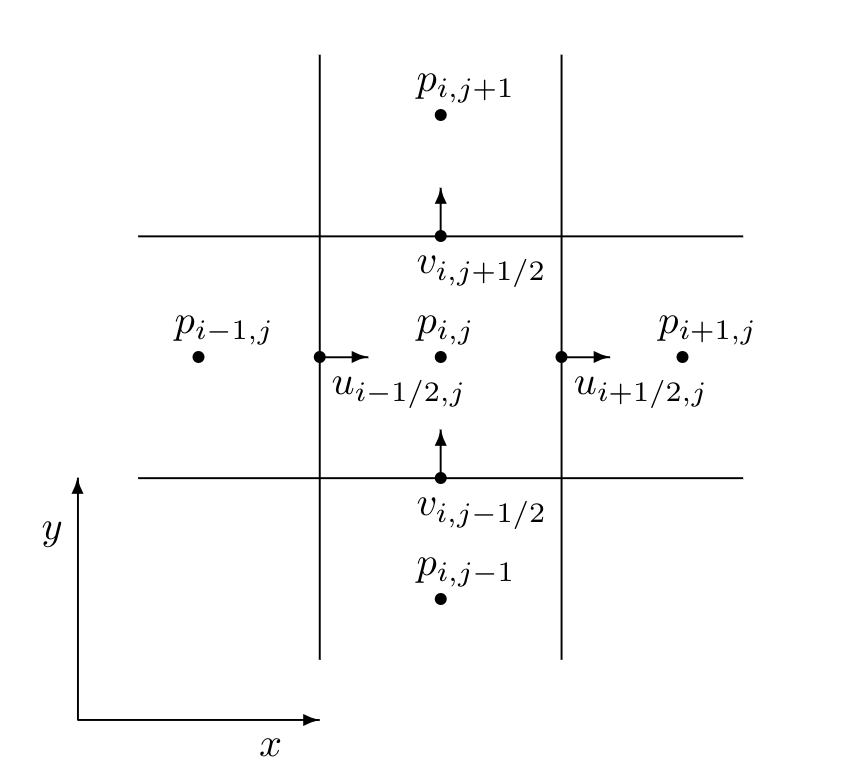
\includegraphics[width=10cm]{image/mac.png}
 \bicaption{二维MAC网格}{2D MAC Grid}
 \label{fig:mac}
\end{figure}

\indent 19世纪由Navier和Stokes提出的纳维-斯托克斯方程方程(Navier-Stokes equations,N-S 方程)是基于物理的流体模拟方法的理论基础\cite{constantin1988navier}。
欧拉网格法\cite{chen2020extended}将流体空间划分为固定的网格单元,在每个网格单元上求解Navier-Stokes方程,以计算流体的速度、压力等物理量在空间和时间上的分布。这种从网格观察流体运动的视角成为欧拉视角。基于网格的数值求解可以分为两步:平流和压力投影\cite{chorin1968numerical}。在平流步骤中,Stam\cite{stam2023stable}提出了无条件稳定的半拉格朗日平流方法。为解决该方法精度低的问题,一系列优化方法被提出\cite{selle2008unconditionally, qu2019efficient, molemaker2008low}。在压力投影步骤中,原始欧拉网格法采用的中心差分方法会导致压力震荡和质量守恒错误,为了解决这一问题,Harlow和Welch\cite{harlow1962particle}在1965年提出MAC(Marker and Cell)方法,与传统网格将所有量存储在网格中心的方法不同,该方法引入交错网格,将压强等标量存储在网格中心、速度等矢量存储在面心,如图\ref{fig:mac}。
\newline
\indent 使用数值求解Navier-Stokes方程需要耗费大量计算资源,Tompson\cite{tompson2017accelerating}提出使用卷积神经网络加速求解Euler方程的方法,使用无监督学习解决线性系统问题,能够实时模拟真实感流体。为了增强神经网络加速Euler流体模拟的灵活性和泛化能力,Dong\cite{dong2019adaptive}提出Smart-Fluidnet,以现有的神经网络为输入,在模拟前输出多个神经网络,模拟时在这些神经网络之间进行动态切换,以满足效率和质量要求。
% \subsection{拉格朗日粒子法}
\newline
\indent 拉格朗日粒子法将流体看作是由相互作用的粒子组成,通过求解粒子的运动方程来模拟流体的运动。其中应用最广泛的是光滑粒子流体动力学方法(SPH,Smoothed Particle Hydrodynamics),该方法由\cite{monaghan2005smoothed}第一次提出。该方法通过保持流体的不可压缩性来求解压强,从而更新粒子位置。基于SPH的不可压缩性求解有很多方法,其中基于假设流体弱可压缩性质的WCSPH法\cite{becker2007weakly}原理和实现较为简单,但稳定性不足,大步长下容易崩溃。基于迭代策略的状态方程法\cite{bender2015divergence}稳定性和仿真速度较好,但精确性较低。为了保证仿真稳定性的同时提升计算效率,Macklin等人将SPH与PBD方法相结合,提出PBF\cite{macklin2013position}方法,该方法不计算压强而直接基于约束修正粒子位置和速度。Kang等人\cite{kang2014incompressible}将无散度条件也视为约束项,进一步提高了PBF方法的稳定性。但由于PBF方法本质上是非物理的方法,因此其视觉真实性不如其它方法。


% \subsection{粒子网格混合法}

\begin{figure}[ht]
 \centering
 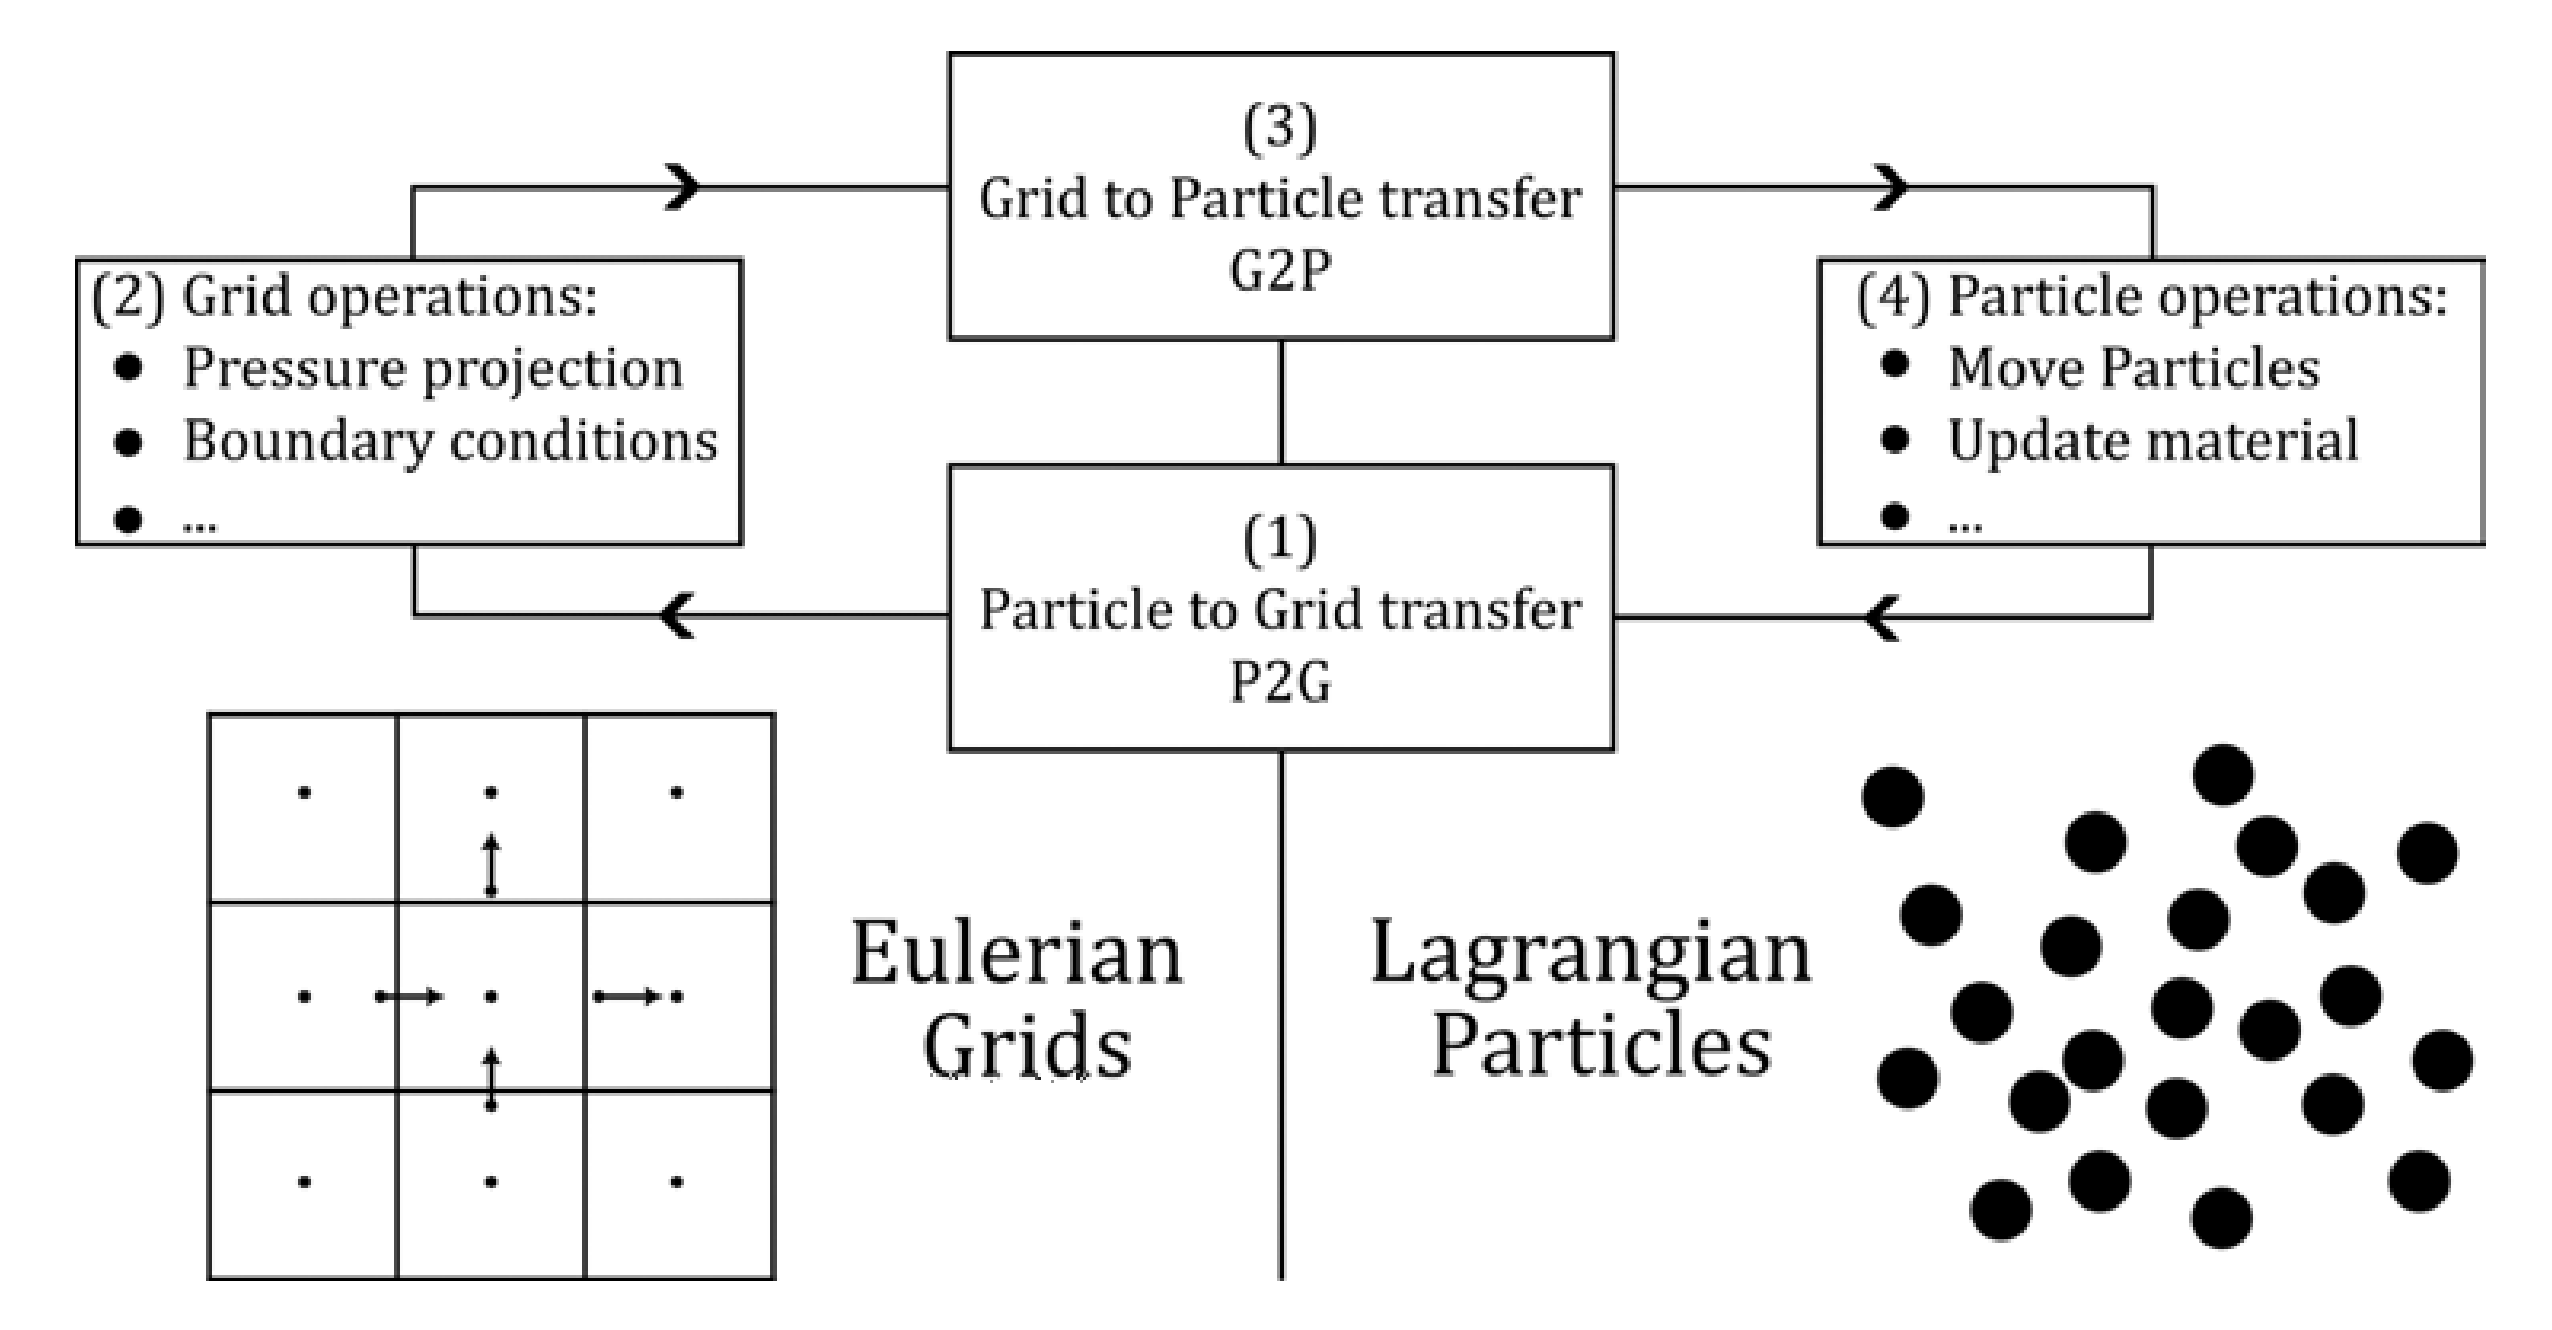
\includegraphics[width=10cm]{image/PIC.png}
 \bicaption{粒子网格混合法步骤}{Particle-grid hybrid method}
 \label{fig:PIC}
\end{figure}

\indent 混合欧拉-拉格朗日方法使用欧拉网格的求解过程,但是基于粒子视角进行模拟。该方法更新粒子状态有四个步骤:粒子转换到网格(P2G)、网格操作、网格转换到粒子(G2P)、移动粒子阶段,如图\ref{fig:PIC}。具体实现为 PIC/FLIP 和 FLIP 方法。其中 PIC/FLIP 将Harlow提出的 PIC 方法\cite{harlow1962particle}和Brackbill提出的 FLIP 方法\cite{brackbill1986flip}相结合,用于在P2G 和 G2P 阶段计算速度,这两个方法的更新结果按照比例混合起来,得到减少能量耗散且噪声变小的流体模拟结果。由于 FLIP 较为不稳定,因此在实际应用中通常使用 0.99 的 FLIP 结果结合 0.01 的 PIC 结果,得到 FLIP99 方案。FLIP方法\cite{zhu2005animating}仅在 G2P 阶段使用,速度从网格转存到粒子时,不再将网格速度直接赋值到粒子速度上,而是将网格增量增加到粒子上一帧的速度。

在上述流体粒子模拟方法中,早期基于数学模型的方法能够很好地模拟水面的性质,但由于缺乏物理原理,真实性不佳。此类方法多应用于极大规模的水面模拟\cite{abbaszadeh2020upwind}和洋流演变,在图形学领域的应用较少。欧拉网格法将流体流过的空间进行离散,将空间划分为网格,在处理大规模流体流动时效率较高,但实现较为复杂,在工程领域具有广泛应用‌\cite{wudeyang2020fluid}。该方法模拟流体时受到网格范围的约束,流体只能在网格内运动。基于拉格朗日视角的模拟方法真实性强,能够模拟流体细节。其中的 SPH 方法在早期通常用于科研的离线模拟,但随着优化方法不断迭代,现在已经能够达到实时模拟的效率。粒子网格混合法将欧拉网格法和拉格朗日粒子法结合起来,后续的优化工作使得该方法稳定性好且无数值耗散问题,但实时性较差\cite{wudeyang2020fluid}。


\section{流体渲染方法研究现状}

目前主流流体渲染方法有流体表面重建方法、光线追踪方法和屏幕空间渲染方法。

\begin{figure}[ht]
 \centering
 \includegraphics[height=6.5cm]{image/anis.png}
 \bicaption{左上:球形粒子,左下:Adams\cite{adams2007adaptively},右:Yu\cite{yu2013reconstructing}}{Top left: spherical particles, bottom left: Adams, right: Yu}
 \label{fig:anis}
\end{figure}

\indent 流体表面重建通过首先重建液体表面,再进行渲染着色得到最终渲染结果。无论是欧拉网格还是拉格朗日粒子法,都需要经过这个步骤进行表面重建。一种被广泛使用的表面重建方法是 Marching Cubes\cite{lorensen1998marching},该方法使用了水平集(Level-Set)\cite{sethian2003level}的思想,将液体表面定义为液体密度等于某个小常数C的点集。欧氏网格法模拟的数据可以直接应用Marching Cubes方法。而对拉氏粒子法生成的数据,则需要根据邻域计算得到的流体密度重建成表面。Adams等人\cite{adams2007adaptively}提出使用基于流体的局部区域信息重构粒子数量和大小的重采样方法,能显著减少需要遍历的粒子数目,减少内存消耗并提升效率。直接通过计算密度重建的表面会出现明显的粒子感,为了缓解这种现象,Yu J 和 Turk G\cite{yu2013reconstructing}将各向异性平滑核作用于球形粒子,使粒子根据位置呈现不同程度的椭球形状,能够取得很好的重建效果,但引入了较大计算量。上述方法的模拟效果见图\ref{fig:anis}。最近开发 Pahi 水模拟管道的研究人员\cite{stomakhin2023pahi}对Yu等人的各向异性方案提出了一种改进方案,进一步减少了不理想的表面伪影。
相比于 Marching Cubes 需要生成显式的网格来表示流体表面,Ray Marching 技术\cite{hart1996sphere, wald2005interactive}提供了一种更为灵活和高效的渲染方式。它直接对密度场进行采样和渲染,从而避免了网格生成的复杂性和性能开销。
\newline
\indent Ray Marching 的核心思想是从相机发射光线,沿着光线方向逐步前进(Marching),并在每一步中采样场景中的密度场或其他场数据。通过累积采样结果,Ray Marching 可以直接渲染出流体的体积效果,支持动态流体、体积光照、折射等复杂效果。这种方法不仅能够处理动态变化的密度场,还可以实现高质量的光学效果,如光线在流体中的散射、反射和透射。尽管 Ray Marching 的计算量较大,但其灵活性和高质量渲染效果使其在流体渲染和体积渲染中得到了广泛应用。通过结合优化技术(如动态步长、早期退出和并行计算),Ray Marching 可以进一步满足实时渲染的需求,成为现代图形学中不可或缺的重要技术。 


\begin{figure}[ht]
 \centering
 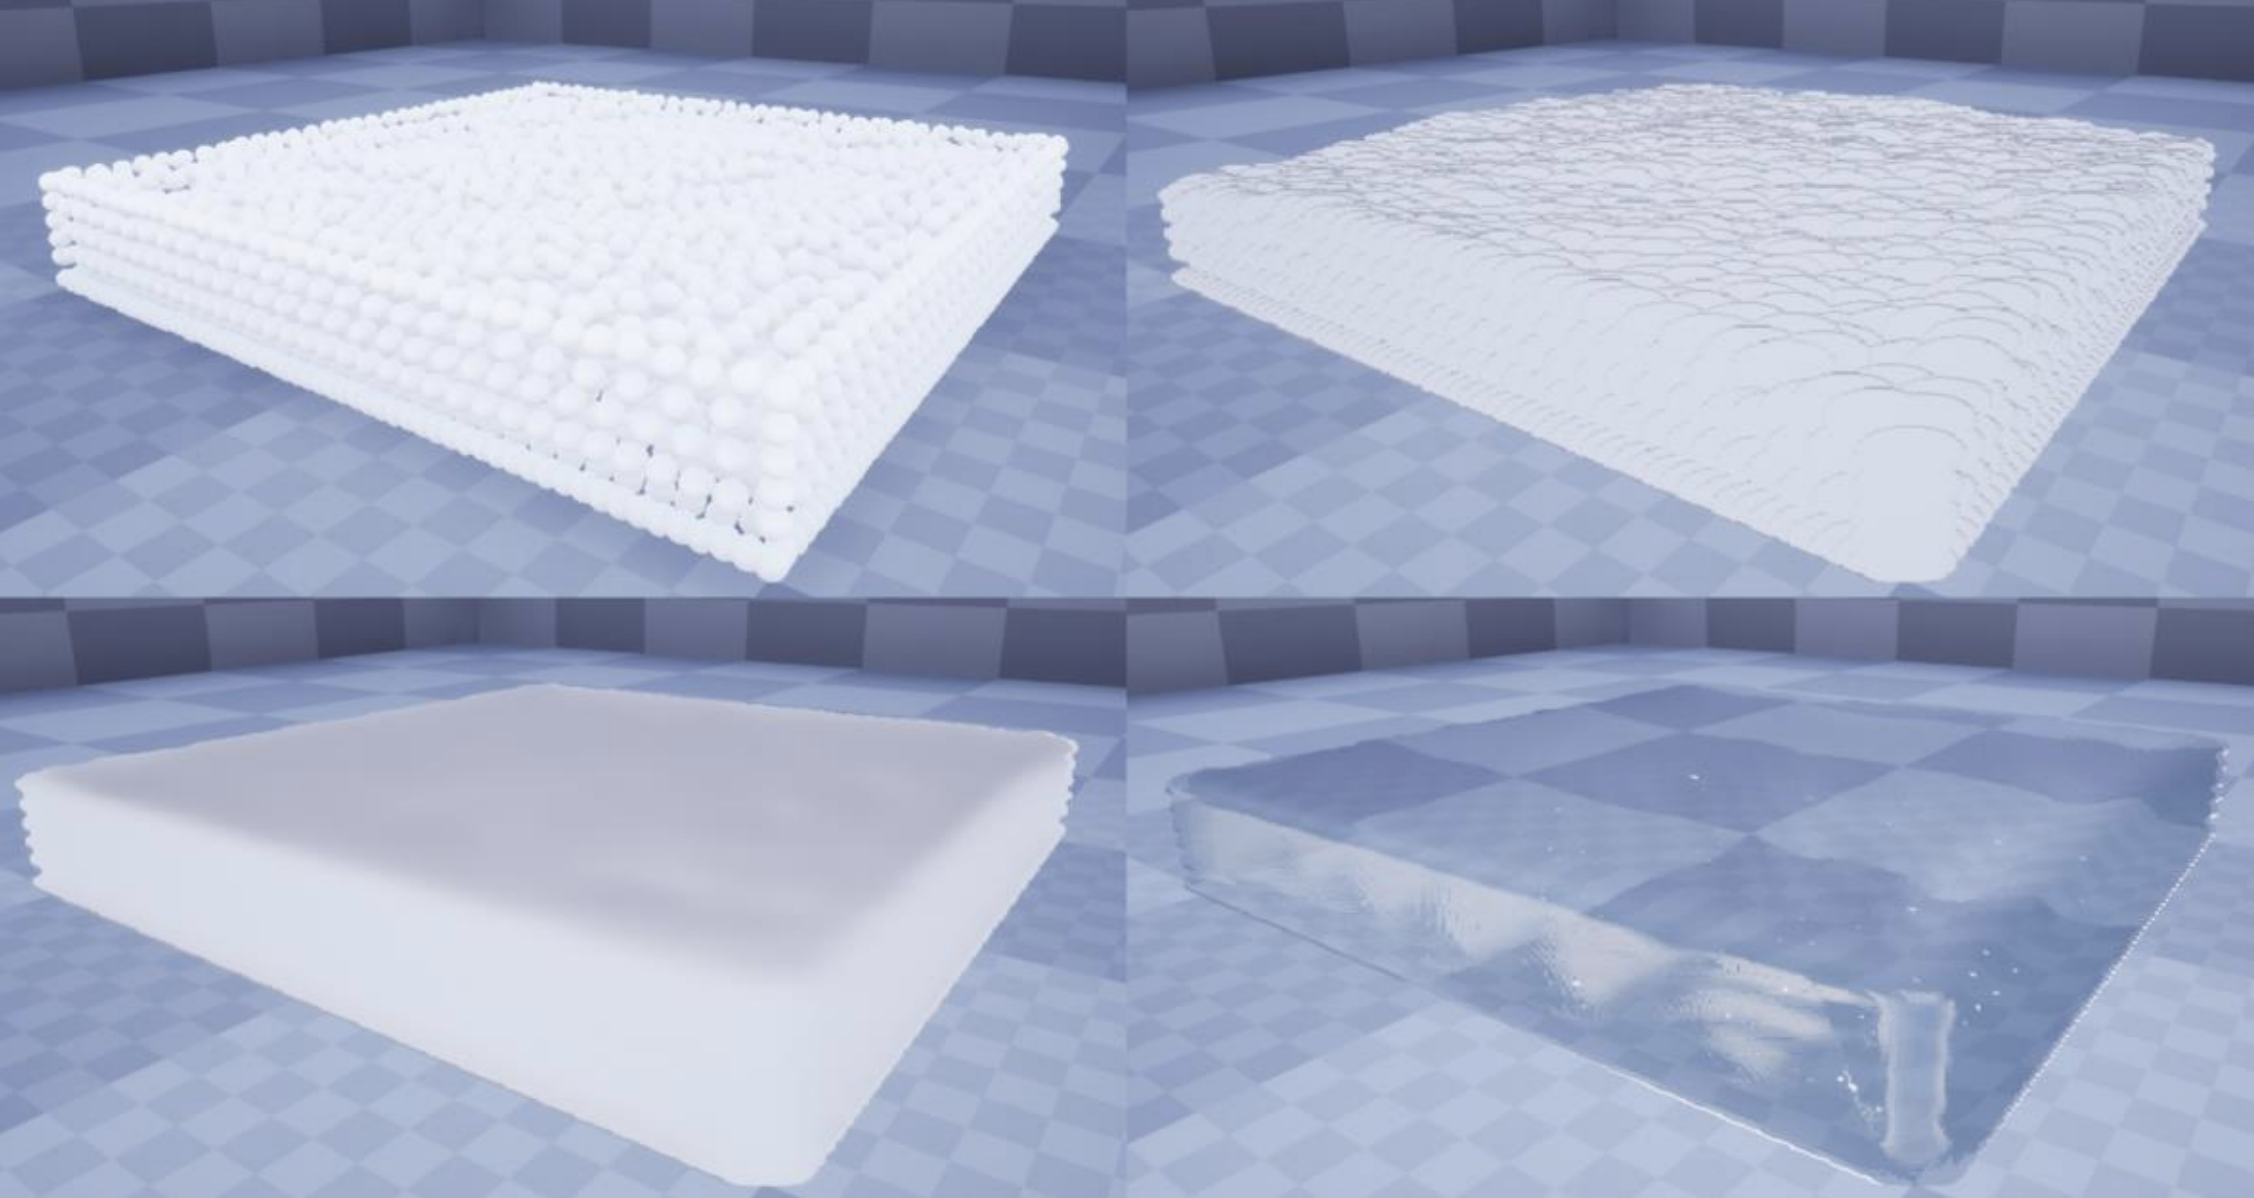
\includegraphics[height=5cm]{image/ssr.png}
 \bicaption{左上图为原始粒子,右上图为未平滑表面,左下图为平滑法线表面,右下图为透明流体渲染效果\cite{1023594216.nh}}{The upper left picture shows the original particles, the upper right picture shows the unsmoothed surface, the lower left picture shows the smoothed normal surface, and the lower right picture shows the transparent fluid rendering effect}
 \label{fig:ssr}
\end{figure}

\indent 真实感流体模拟和渲染在计算上的开销是巨大的,屏幕空间渲染\cite{van2009screen}给出了粒子渲染的一种新思路。这类方法舍弃了流体表面的匹配和重建的传统思路,给出了简单、实时、低消耗的实现方案。主要思路是通过流体粒子在屏幕空间的深度纹理和厚度纹理重建法线,再结合光线追踪操作对表面进行着色。在进行深度纹理还原法线的步骤中,不经过平滑会得到粒子感较强的流体表面,因此对屏幕空间渲染算法的改进涉及多种滤波器方法\cite{muller2007screen, bagar2010layered, neto2017real, truong2018narrow, oliveira2022narrow}。其中Neto L S R\cite{neto2017real}提出使用双边高斯滤波进行深度图的模糊,取得了较好的效果,如图\ref{fig:ssr}。在对重建得到的法线进行透明水体材质的渲染时,几乎所有系统都采纳了一种名为 Cook-Torrance BRDF\cite{cook1982reflectance}的反射模型。经过较多研究进行优化\cite{schlick1994inexpensive, burley2012physically},该方法已经成为一套成熟的实时渲染解决方案。
\newline
\indent 以Marching Cubes为代表的传统表面重建方法在 GPU 并行化上还有较大优化空间,整体算法计算量较大,无法实时渲染大规模流体场景。使用光线追踪技术进行流体渲染的计算量相对较大,但能够产生足够平滑和具有真实感的效果。屏幕空间渲染方法速度快,能够大大减少计算资源的消耗,尤其适合实时渲染应用,但渲染质量不如光线追踪进行流体渲染的效果。

\section{低功耗渲染技术的研究进展}

\indent 在流体仿真方面,我们对针对SPH算法进行低功耗优化的工作做了调研,目前已有较多针对其算法效率进行优化的技术手段。SPH的各阶段计算都需要邻域粒子求和,大规模流体模拟中邻域粒子查找成为限制性能的瓶颈之一。一种效果较好的优化方法是粒子索引压缩存储方法\cite{band2020compressed, horvath2012real, winchenbach2020multi},该方法将粒子在网格中的位置按照哈希值存储,并用偏移量代替粒子索引,从而降低空间开销并提升邻域查找速度。同时,使用GPU进行并行加速能进一步提升计算效率。目前最新的邻域搜索算法是TENCENT GAMES工作室\cite{liu2023building}提出的基于 GPU 的位掩码方法,该方法采用32位无符号整数编码粒子列表,重组相邻单元,遍历粒子生成位掩码标记邻域粒子,利用快速遍历算法依位掩码查找,提升效率并节省内存。
\newline
\indent 另一种从全局减少计算量大方法是自适应分辨率SPH法,最早由Adams\cite{adams2007adaptively}提出,该方法在流体近处使用高分辨率粒子来保证视觉质量,而在其他位置使用低分辨率降低运算量。Solenthaler\cite{solenthaler2011two}、Orthmann\cite{orthmann2012temporal}和Winchenbach\cite{winchenbach2021optimized}等人陆续对该方法进行了优化,有效提高了自适应分辨率SPH法的稳定性。但该方法无法使用GPU加速,且稳定性仍有待完善。
\newline
\indent
在流体渲染方面,我们对Ray Marching方法的低功耗优化工作进行了调研。由于直接对所有粒子进行Ray Marching计算会产生很大的计算开销。Fraedrich等人\cite{fraedrich2010efficient}在模拟域中将粒子重新采样到临时均匀的 3D 网格中,并在相机空间中使用透视网格,从而减少要处理的粒子数量并降低内存消耗。Kanamori 等人\cite{kanamori2008gpu}通过直接计算视线和粒子的交点来生成等值面,以避免临时网格的内存消耗。Xiao 等人\cite{xiao2017real}通过光栅化粒子来快速获取光线投射的入口,以帮助光线跳过相机到可见粒子区域之间的大量空白。Biedert 等人\cite{biedert2018direct}则提出了一种基于各向异性平滑核的自由表面交集光线追踪方案,有效地减少了候选粒子的数量。
TENCENT GAMES工作室\cite{liu2023building}提出简化版 Whitted 风格光线追踪算法,该算法对不重要的光线分支进行修剪,减少了数据传输量,并基于 GPU 进行加速,渲染效率较高。

% \input{RelateWork}

\chapter{基于粒子的快速流体仿真方法}

在计算机图形学和物理模拟中,基于粒子的流体仿真方法因其灵活性和可扩展性,被广泛应用于计算机动画、游戏和物理建模领域。SPH(Smoothed Particle Hydrodynamics)是一种常用的粒子方法,通过核函数(Kernel Function)对粒子属性进行平滑化插值,以实现流体特性的逼真模拟。本章节将详细介绍 SPH 流体模拟的基本原理,并探讨在移动端环境中的计算优化技术,尤其是邻域搜索的优化策略,如计数排序(Count Sort)和哈希存储(Hash Grid)。

\section{SPH 流体模拟的实现原理}

\subsection{流体动力学建模}

在SPH方法中,流体被表示为一组离散的粒子,每个粒子都携带物理属性,如位置、速度、密度和压力等。根据流体的特征,一般通过不可压缩性条件\eqref{con:incompition}和纳维-斯托克斯方程\eqref{con:Momentum}来近似定义流体的动力学行为。
% ,包括动量方程\eqref{con:Momentum}(即纳维-斯托克斯方程)、无散度条件\eqref{con:incompition}、质量守恒方程\eqref{con:Continuity}和状态方程\eqref{con:State}
对流体的模拟实际上就是求解每帧粒子的位置,每个粒子的位置变化的影响因素有体积力(如重力、离心力)和流体内部粒子的相互作用力,包括不可压缩性约束的压强作用、流体粘性力。
%NS方程
流体动力学的核心是动量方程,它本质上是牛顿定律$\vec{F}=m\vec{a}$的形式,描述了粒子受力后的加速度变化。SPH 采用如下动量方程,本质上是不可压缩Navier-Stokes偏微分方程:
\begin{equation}
    \frac{d v_i}{dt} = -\frac{1}{\rho_i} \nabla P_i + \nu \nabla^2 v_i + f\label{con:Momentum}
\end{equation}
其中,$-\frac{1}{\rho_i} \nabla P_i$ 是压力梯度项,$- \nu \nabla^2 v_i$ 是粘性力项,$f$ 是外部合力的量化数据,如重力。SPH通过NS方程和不可压缩性条件来描述流体运动,NS方程等式右端的压力梯度项由流体的不可压缩性\eqref{con:incompition}约束。通过离散化求解将SPH的实现过程分解为三项独立求解:压力求解、粘性求解和外力求解,本文系统实现方法也将以此为基础构建流体模拟方法。

\begin{equation}
    \frac{d\rho}{dt} = -\rho\nabla \cdot \mathbf{u} = 0\label{con:incompition}
\end{equation}

在求解过程中,在只有重力的情况下,外力的方向大小固定,可通过计算加速度直接更新粒子速度和位置进行求解。而要求解NS方程等式右边的压力梯度项和粘性力项,则需要先求解流体内的压力场和速度场。因为SPH属于粒子系统的插值方法,在空间任意位置计算仅由离散粒子位置定义的场量,通过对称的平滑内核在每个粒子的局部邻域内计算场量值。如标量场量$A$在位置$r$处通过公式\eqref{con:A_S}插值计算。

\begin{equation}
    A_S(r) = \sum_j V_j A_j \nabla W(r - r_j, h)\label{con:A_S}
\end{equation}

其中$j$遍历所有粒子,$V_j$,$r_j$, $A_j$分别为粒子$j$的质量体积、位置和场量,$W(r,h)$是核心半径为$h$的平滑内核。$W$需要满足是偶函数且归一化($\int W(r)dr=1$)。在公式\eqref{con:A_S}中,每个粒子都具有一定体积$V_i=m_i/\rho_i$。在一般模拟过程中,粒子质量$m_i$保持恒定且所有粒子质量相同,但密度$\rho_i$会发生变化,所以需要在每个时间步重新计算。
由于在NS方程中包含对场量的梯度和拉普拉斯算子的求解,对公式\eqref{con:rho_s}进一步求导可得$A$的梯度\eqref{con:nablaA_S}和拉普拉斯算子\eqref{con:nabla2A_S}:

\begin{equation}
    \nabla A_S(r) = \sum_j m_j \frac{A_j}{\rho_j} \nabla W(r-r_j,h)\label{con:nablaA_S}
\end{equation}
\begin{equation}
    \nabla^2 A_S(r) = \sum_j m_j \frac{A_j}{\rho_j} \nabla^2 W(r-r_j,h)\label{con:nabla2A_S}
\end{equation}

结合上述基本原理,将相关量代入公式\eqref{con:A_S}可以得到位置$r$处的密度公式\eqref{con:rho_s},压力梯度项公式\eqref{con:pressure},粘性力公式\eqref{con:viscosity}:

\begin{equation}
    \rho_S(r) = \sum_j m_j \frac{\rho_j}{\rho_j}W(r-r_j,h)=\sum_jm_jW(r-r_j,h)\label{con:rho_s}
\end{equation}
\begin{equation}
    F_i^{pressure} = -\frac{1}{\rho_i} \nabla P_i =  -\sum_j m_j \left( \frac{P_i + P_j}{2\rho_j} \right) \nabla W(r_i - r_j, h)
    \label{con:pressure}
\end{equation}
\begin{equation}
    F_i^{viscosity} = - \nu \nabla^2 v_i =  \mu \sum_j m_j \frac{(v_j - v_i)}{\rho_j} \nabla^2 W(r_i - r_j, h)
    \label{con:viscosity}
\end{equation}

SPH方法的稳定性、准确性和速度在很大程度上取决于平滑核函数的选择上。通常情况下选择具有二阶插值误差的核函数,在满足偶函数且归一化限制条件下,可以自由设计用于特定目的的内核。提出SPH方法的作者\cite{muller2003particle}规定了计算密度、压力和粘度时可选择的核函数,如图\ref{fig:threekernel}。除了压力和粘度的计算外,一般都选择$W_{poly6}$核函数进行计算。由图\ref{fig:threekernel}中最左侧实线所示,随着距离的减小,其一阶导数(梯度)越来越小甚至趋近于$0$,若用此函数计算压力,当两个粒子接近重合时,将两个粒子分开的力非常小,这违背了流体的不可压缩性,不符合实际情况,因此选择更加尖锐的$W_{spiky}$核函数计算压力。在粘性力的求解中,需要对核函数求拉普拉斯算子, $W_{poly6}$和$W_{spiky}$核的拉普拉斯算子可能会变成负值,从而导致两个相互靠近的粒子相对速度增加,在粒子数量相对较少时会导致稳定性问题。因此使用$W_{viscosity}$核函数,其拉普拉斯算子处处为正,能够显著提高模拟稳定性。上述三种核函数及其导数和拉普拉斯算子推导公式见附录\ref{formula}。

\begin{figure}[ht]
 \centering
 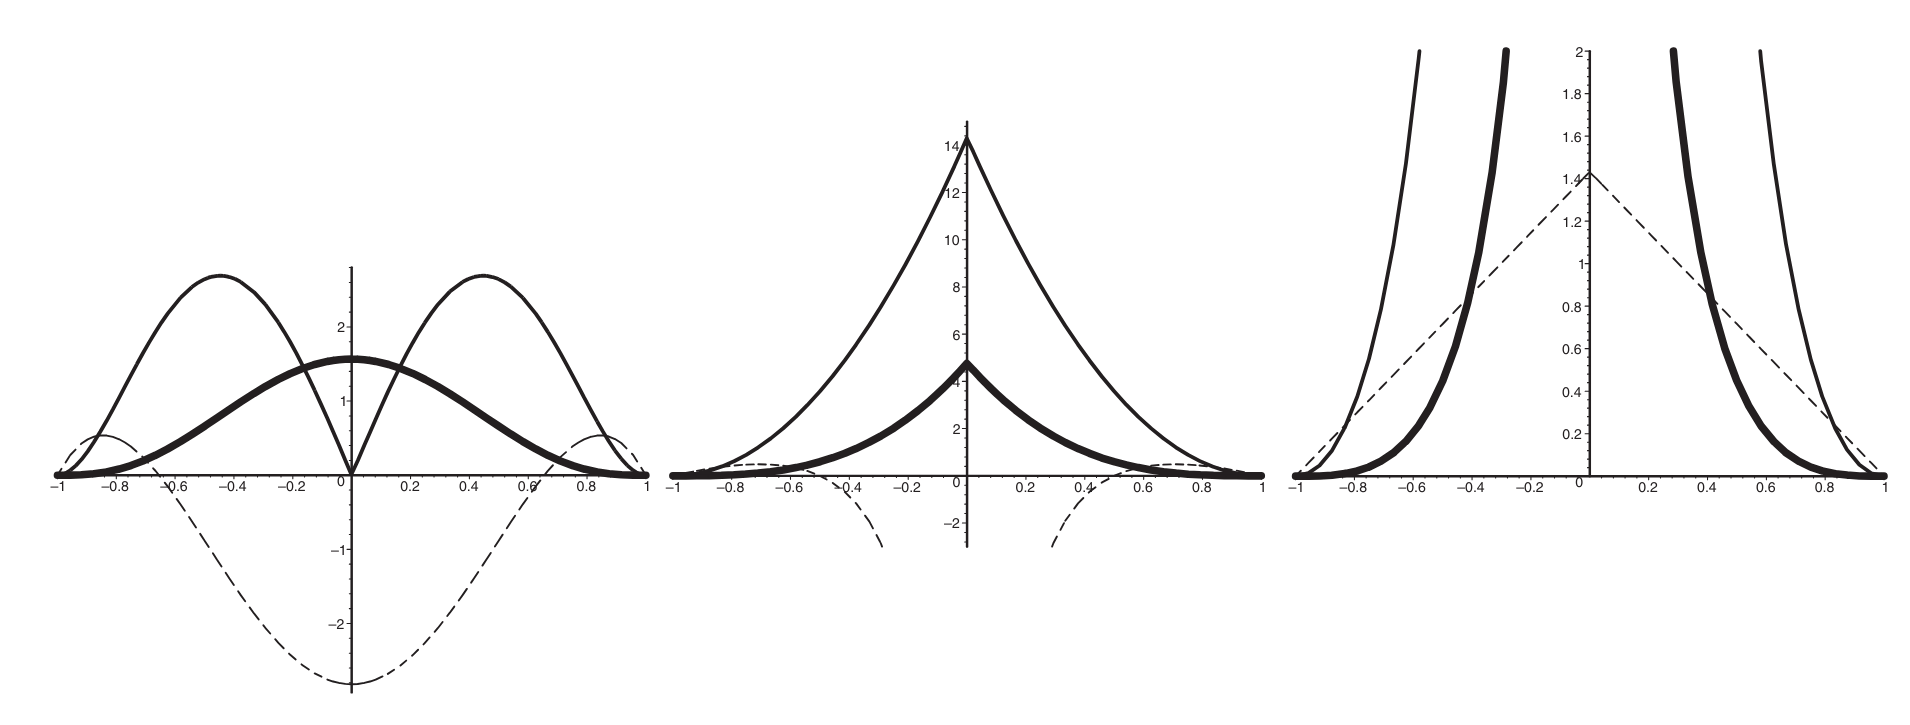
\includegraphics[height=5cm]{image/threekernel.png}
 \bicaption{三种平滑核,从左到右分别为$W_{poly6}$,$W_{spiky}$,$W_{viscosity}$。粗线表示基本核函数,细线表示梯度,虚线表示拉普拉斯算子}{The three smoothing kernels $W_{poly6}$, $W_{spiky}$, $W_{viscosity}$(from left to right)}
 \label{fig:threekernel}
\end{figure}




在进行流体仿真时,每帧计算以上一帧结果为输入,通过如图\ref{fig:pipeline1}的计算流程求解NS方程中的速度并更新流体粒子的位置。结束NS方程的求解后,根据当前系统的需求将该帧计算得到的粒子位置数据结果进行实时渲染,或将所有帧模拟结果存储到硬盘进行统一分析、处理或离线渲染。

\begin{figure}[ht]
 \centering
 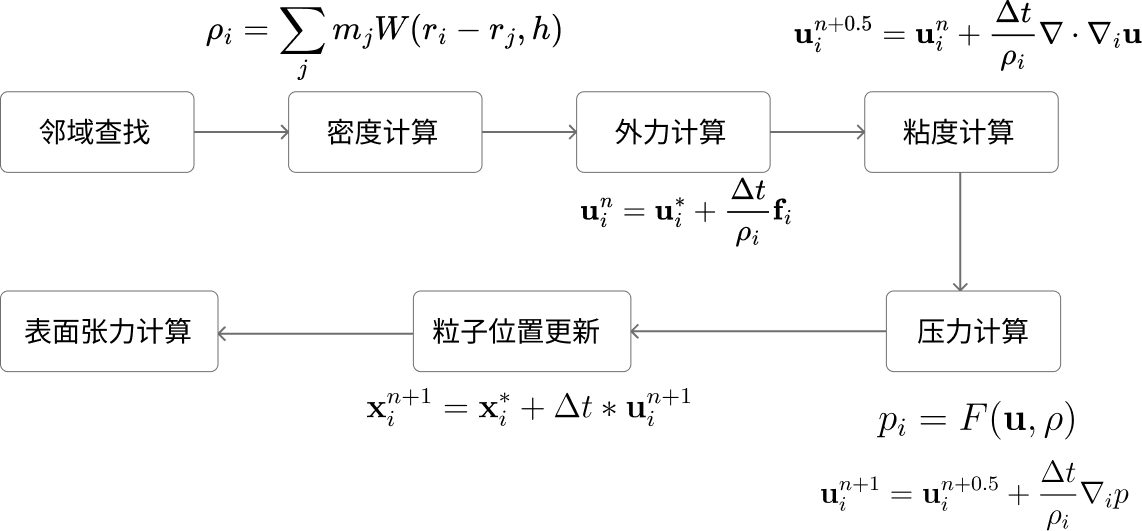
\includegraphics[height=5cm]{image/pic1.png}
 \bicaption{SPH法实现流体模拟的基本流程}{The basic pipeline of fluid simulation by SPH method}
 \label{fig:pipeline1}
\end{figure}

在图\ref{fig:pipeline1}中描述了一般SPH方法的基本流程。其中,每帧计算的第一步即查找并存储每个粒子的邻域粒子,用于后续计算,邻域查找过程的时间和空间复杂度较高,在实时应用中需要进一步优化以保证仿真效率。求解NS方程的各项力之前要预先计算每个粒子的质量密度,可通过每个粒子的邻域粒子的质量分布计算得到。之后分别对外力、粘性力和压力进行计算,采用上述核函数保证计算结果的稳定性。最后对粒子位置进行更新。传统SPH方法不包含流体表面张力的求解,但实际应用中需要考虑该因素。

%  SPH 方法计算NS方程中的压力梯度项公式如下\eqref{con:pressure}:

% \begin{equation}
%     F_i^{pressure} = -\frac{1}{\rho_i} \nabla P_i =  -\sum_j m_j \left( \frac{P_i + P_j}{2\rho_j} \right) \nabla W(r_i - r_j, h)
%     \label{con:pressure}
% \end{equation}

% 粘性力计算如下\eqref{con:viscosity}:

% \begin{equation}
%     F_i^{viscosity} = - \nu \nabla^2 v_i =  \mu \sum_j m_j \frac{(v_j - v_i)}{\rho_j} \nabla^2 W(r_i - r_j, h)
%     \label{con:viscosity}
% \end{equation}
% 其中 $\mu$ 是粘度系数,用于控制流体的粘滞性。
% 质量守恒方程表示在流体流动过程中任意一点的质量不会凭空产生或消失,主要用于流体密度计算。在 SPH 方法中,密度 $\rho_i$ 由核函数加权计算得出:
% \begin{equation}
%     \rho_i = \sum_{j} m_j W(r_i - r_j, h)\label{con:Continuity}
% \end{equation}
% 其中,$m_j$是邻域粒子$j$的质量,$W(r_i - r_j, h)$ 是以光滑长度 $h$ 为参数的核函数,$r_i$, $r_j$ 分别是粒子 $i$ 和 $j$ 的位置。该公式表明,某粒子 $i$ 的密度由其周围粒子的质量和核函数的贡献共同决定。为了保证流体不可压缩性,需要对密度进行严格约束。
% 为了计算流体的压力,SPH 方法通常使用状态方程:
% \begin{equation}
%     P_i = k (\rho_i - \rho_0)\label{con:State}
% \end{equation}
% 其中 $k$ 为刚度系数(Stiffness Constant),$\rho_0$ 是目标密度(Rest Density)。状态方程用于保证流体的不可压缩性,即粒子的密度应始终接近 $\rho_0$。


\subsection{SPH方法具体实现流程}

\begin{figure}[ht]
 \centering
 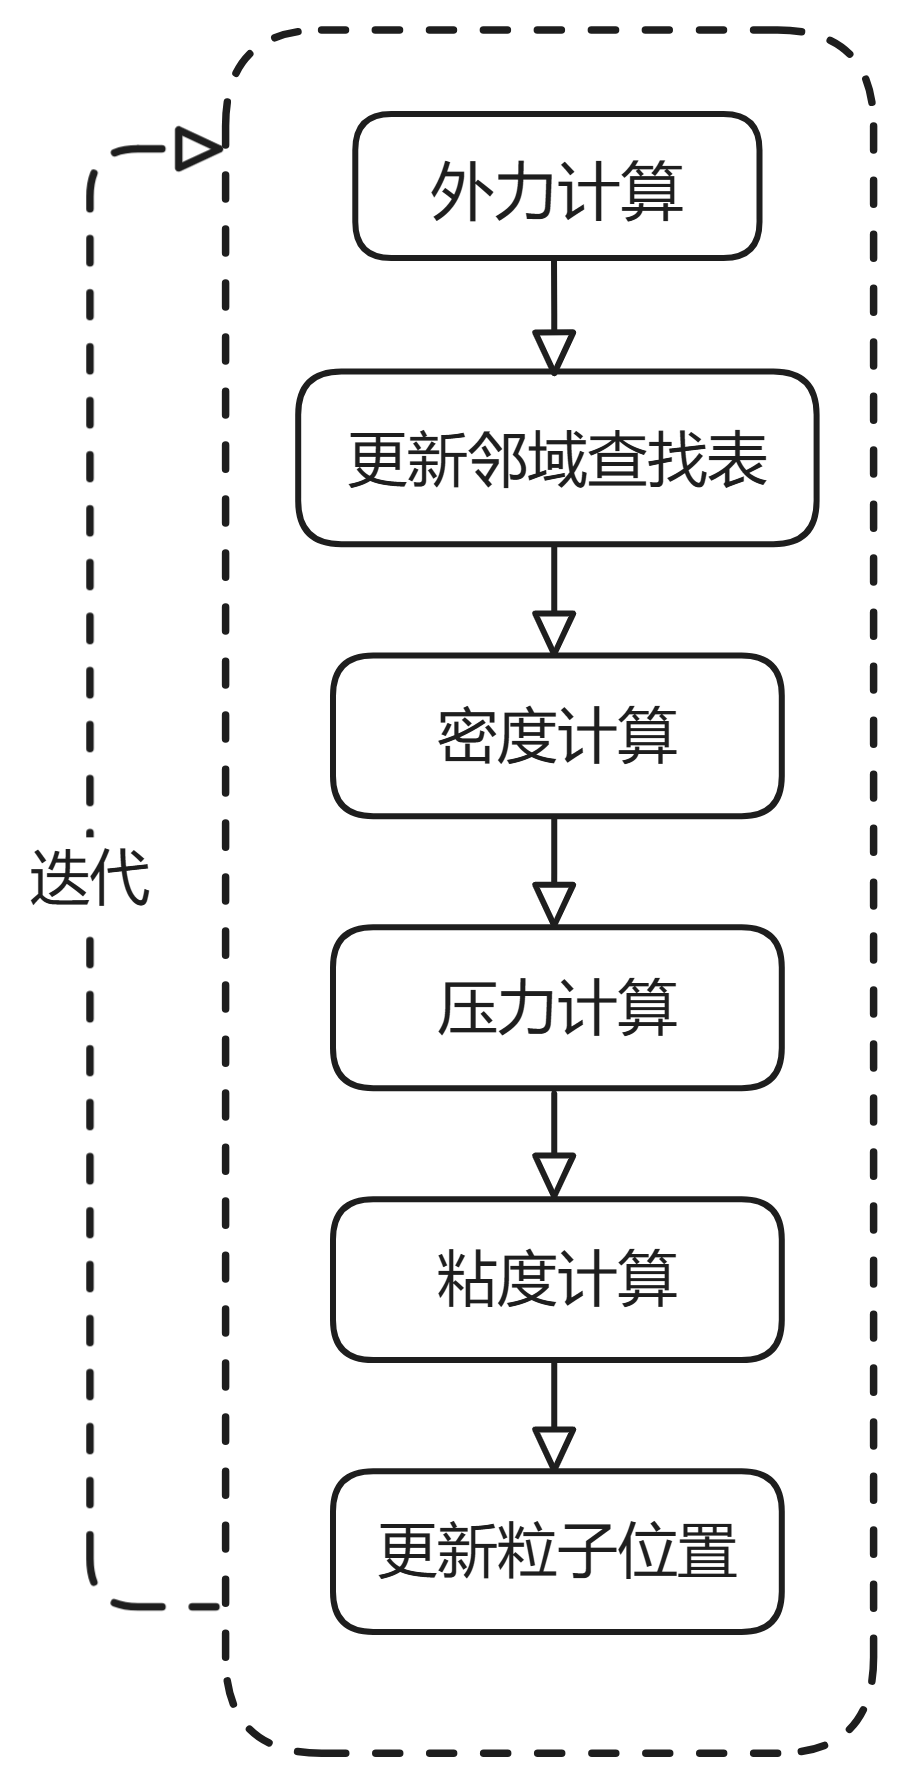
\includegraphics[height=8cm]{image/pic2.png}
 \bicaption{本文系统实现流体模拟的基本流程}{The basic process of fluid simulation implemented by the system in this paper}
 \label{fig:pipeline2}
\end{figure}

本文采用的流体模拟方法基于传统SPH,但在流程和具体求解方法上进行了调整和优化,总体流程如图\ref{fig:pipeline2}。
为提高流体粒子模拟的稳定性和真实感,系统在每帧内设置迭代次数,每次迭代即对上图流程进行一次串行遍历,针对具体对象的计算通过ComputerShader在GPU并行处理。在每个子步中,首先对所有粒子根据其当前位置、速度和重力计算预测位置和速度,将得到的新粒子位置和速度传输到下一步骤。在更新邻域查找表步骤中进行空间散列更新和排序,通过哈希存储和并行计数排序使得每次邻域查找的时间复杂度为$O(1)$,这部分具体解释见章节\ref{optim}。
在不可压缩性求解过程中,仅依靠简单的密度和压力项无法防止粒子聚集。一个粒子可能通过强烈吸引少量邻居达到目标密度值,导致流体分离成独立团簇而缺乏连续性和真实感。同时,由于原始方法没有针对流体表面粒子的特殊情况进行专门处理。如图\ref{fig:surface}所示,绿色粒子的邻域完整,而位于流体表面的红色粒子在空气中没有相邻粒子,导致其密度被低估,进而导致流体表面的粒子有向空气中移动的趋势。以空气中的水滴为例,当其落下时,内部粒子会四散开来,而正常的水滴由于表面张力的作用会聚集在一起落下。为了解决上述粒子聚集问题和表面张力问题,我们对密度和压力的求解进行了改进。
\begin{figure}[ht]
 \centering
 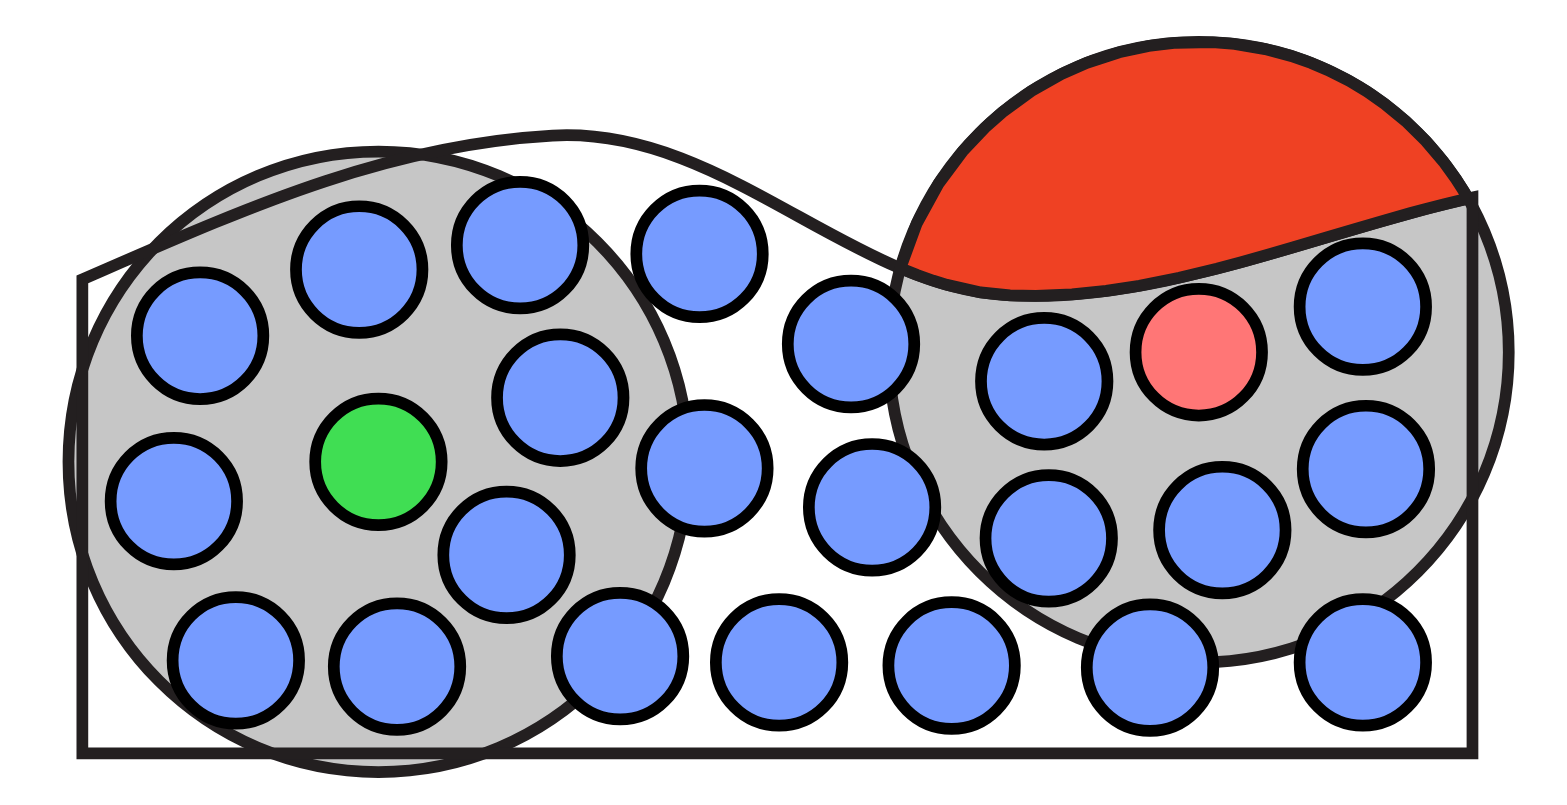
\includegraphics[height=5cm]{image/bounder.png}
 \bicaption{流体表面问题}{Fluid surface problem}
 \label{fig:surface}
\end{figure}

我们参考了\cite{clavet2005particle}提出的近密度和近压力方法。该方法增加一个额外的压力,即近压力,该额外压力通过近密度计算,近密度计算相比原始密度计算采用了更加尖锐的核函数,如图\ref{fig:nearkernel}。
\begin{figure}[ht]
 \centering
 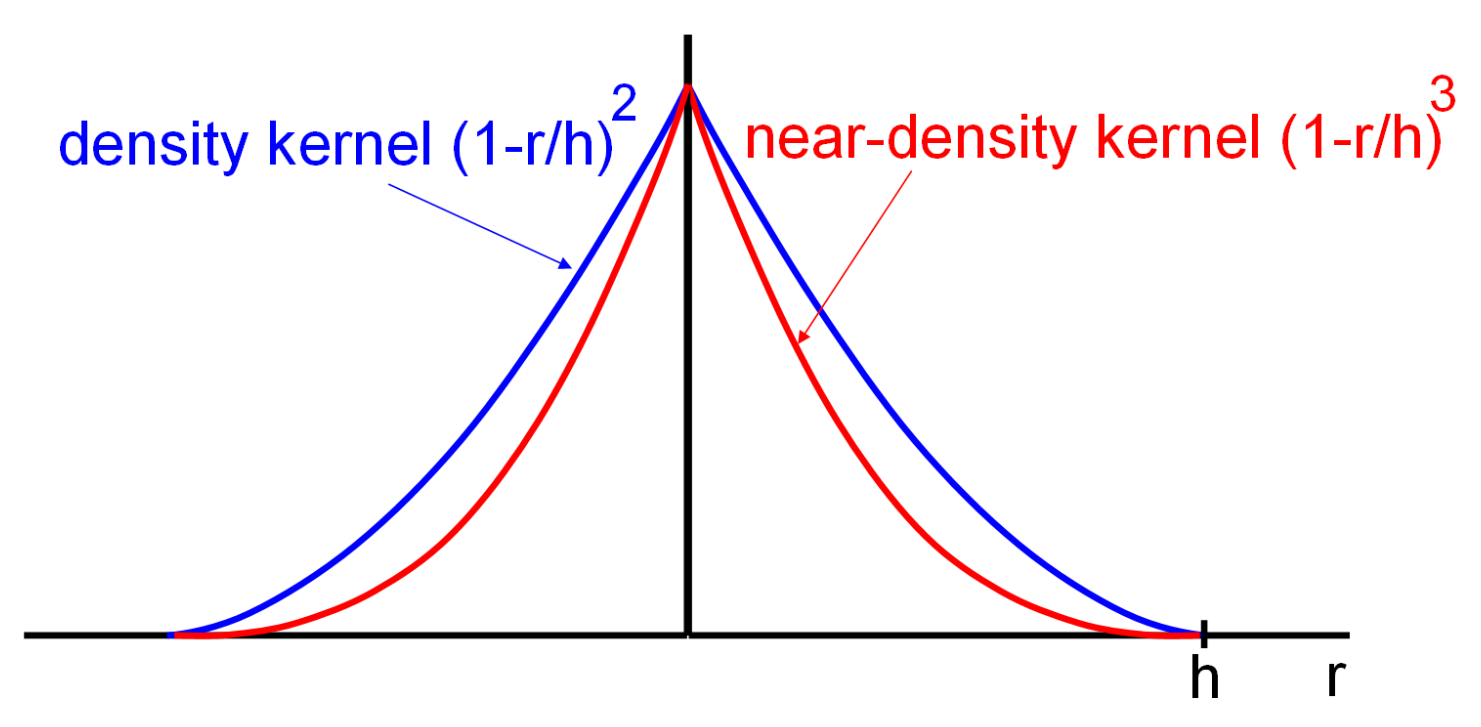
\includegraphics[height=5cm]{image/nearkernel.png}
 \bicaption{近密度核和原始密度核图像的对比}{Comparison of near density kernel and original density kernel images}
 \label{fig:nearkernel}
\end{figure}
为了让近压力完全是排斥力,将近压力定义为$P_i^{near}=k^{near}\rho_i^{near}$,这与原始压力的定义类似,但静止密度为零,它在粒子间相互作用中提供额外的排斥力,防止粒子过度聚集。具体算法中,对每个粒子计算密度、近密度、压力和近压力,然后更新预测粒子位移。当粒子位置的密度小于指定密度时,压力和近压力对邻居粒子的作用不同。压力将邻居粒子向该粒子拉近,近压力则将邻居粒子推离,从而避免粒子聚集。压力和近压力对不同距离的邻居粒子的影响也不同。较远的邻居粒子受近压力影响小。这是因为近压力的核函数$(1-\frac{r_{ij}}{h})^2$ 随着粒子间距离$r_{ij}$的增大而迅速减小,所以对于距离较远的邻居粒子,近压力的作用相对较弱。在压力的吸引作用下,较远的邻居粒子更容易移动,因为它们受到的近压力排斥较小,而压力的吸引作用相对更显著 。最近粒子受到近压力的排斥作用相对较强,这种平滑排斥使得最近粒子不会过度靠近中心粒子。这种排斥作用虽然是短距离的,但却间接导致了长距离的吸引效果。因为较远粒子在压力吸引下向中心粒子靠近时,最近粒子的排斥使得较远粒子之间的相对位置发生变化,从而在宏观上表现出一种长距离的吸引效果,从而形成表面张力效果。使用近密度和近压力方法,粒子能与所有紧邻邻居保持等距,避免粒子聚集,也能使远距离粒子不至于太分散,模拟表面张力效果。

在对粘度进行计算时,原始基于物理的粘性计算稳定性差且计算成本较高,我们选用XSPH\cite{schechter2012ghost}中的非物理的粘性计算方法。该方法能够对粒子速度进行局部平滑处理,从而有效减少粒子的震荡情况。其实现方式简单且效率更高,并且具有良好的稳定性。该粘性方法对应的速度场平滑化公式如下\eqref{con:XSPH}。应用该粘度力方程,意味着随着时间的推移,每个粒子的速度会变得更像它的邻居,邻居对该粒子的影响由粘性强度系数$\varepsilon$和粘度核函数(本系统使用$W_{poly6}$核函数)控制。
\begin{equation}
    \mathbf{u} _i^{n+0.5}=\mathbf{u} _i^n+\varepsilon \sum_j \frac{m_j}{\rho_j}(\mathbf{u}_j^n-\mathbf{u}_i^n)W(r_{ij},h)
    \label{con:XSPH}
\end{equation}

最后更新粒子位置时进行碰撞检测,在触碰到边界时将粒子速度反向并乘以阻尼系数。经上述步骤模拟的流体粒子每30帧共600帧图像如图\ref{fig:paritcleSim}所示,其中粒子用点精灵代替,颜色根据速度大小进行渲染。
\begin{figure}[ht]
 \centering
 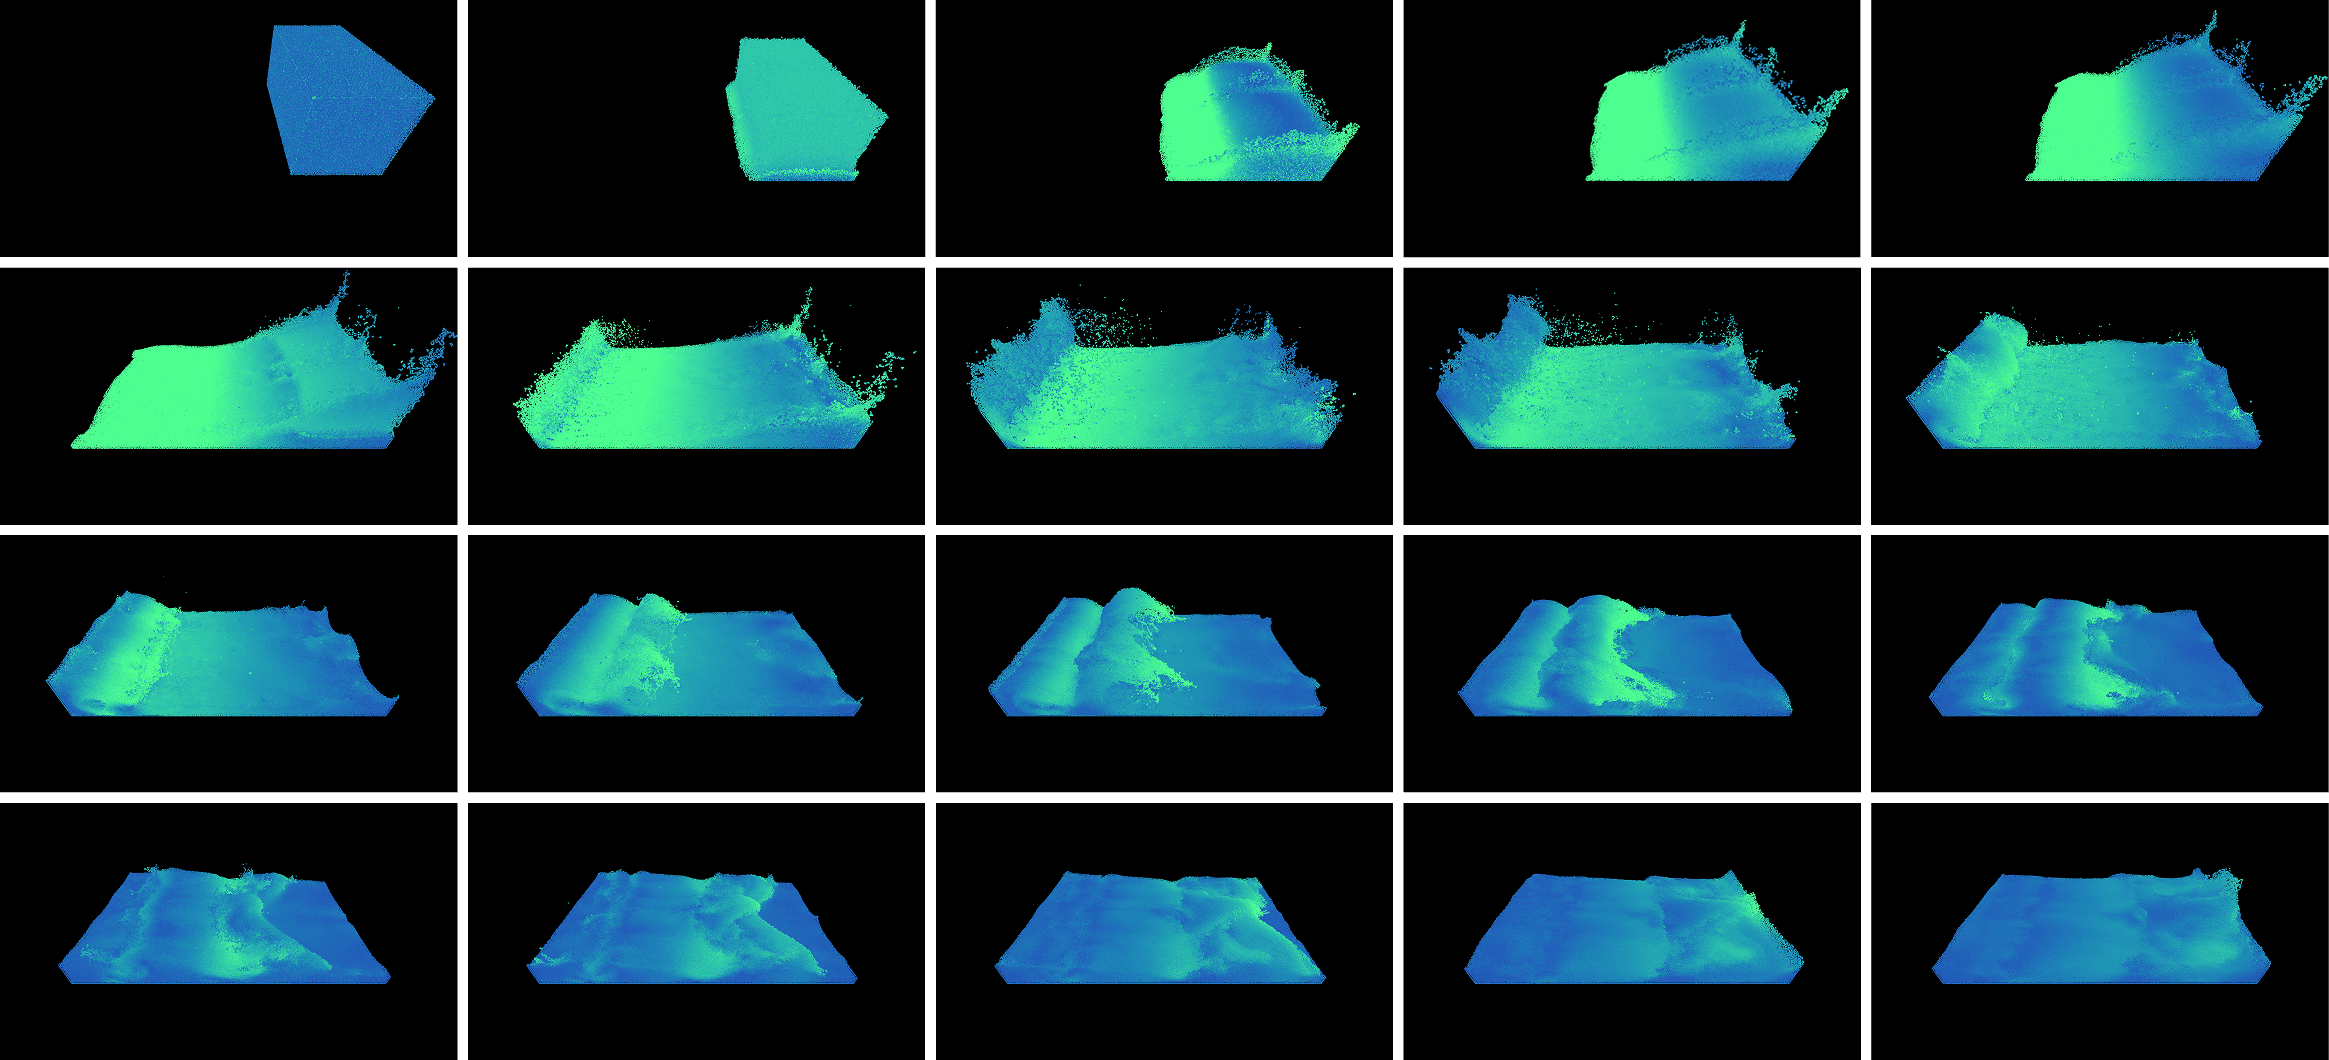
\includegraphics[height=5cm]{image/pic3.png}
 \bicaption{流体粒子模拟逐帧图}{Fluid particle simulation frame-by-frame diagram}
 \label{fig:paritcleSim}
\end{figure}


\section{移动端的计算优化}
\subsection{存储空间邻域搜索优化}\label{optim}

\subsubsection{邻域搜索数据结构优化}
在传统SPH方法中对于当前粒子的密度、压力和粘度等的计算需要通过对当前粒子的邻域粒子属性进行求和计算。通过设置一个邻域半径,对每个粒子,遍历所有其他粒子,若粒子与当前粒子的距离小于该邻域半径,就将该粒子的物理属性值累加至当前粒子该物理属性上进行求和计算。当粒子数目增加时,遍历所有粒子的方法便难以满足实时要求。一种可参考的优化方法是建立一个均匀网格,这是一种可能的最简单的空间细分方式,还有其他更复杂的结构如层次化网格,但我们在此不做讨论。均匀网格将模拟空间细分为大小均匀的网格单元。将网格中单元大小设置为邻域半径,这样当在三维空间寻找邻域半径内的粒子时,只需考虑圆心周围的27个单元格。该方法在全局内存中使用两个数组:一是网格计数器数组gridCounters,用于存储到目前为止每个单元中的粒子数量。在每一帧开始时,它被初始化为零。二是网格单元数组gridCells,用于存储每个单元的粒子索引,并且为每个单元中固定的最大粒子数量预留了空间。这种方法假定每个网格单元中粒子的最大数量是固定的,并且不支持网格动态变化,粒子只能在初始化时规定的网格内部运动。

基于这种方法,我们考虑优化其数据结构,通过设置与粒子数量等长的额外两个数组,使得不需要提前知道网格的尺寸,粒子可以传播到世界上任何地方。下面将以图\ref{fig:gridParticle}所示的网格和粒子分布阐述本文系统在邻域搜索的数据结构上优化的具体步骤。

\begin{figure}[ht]
    \centering
    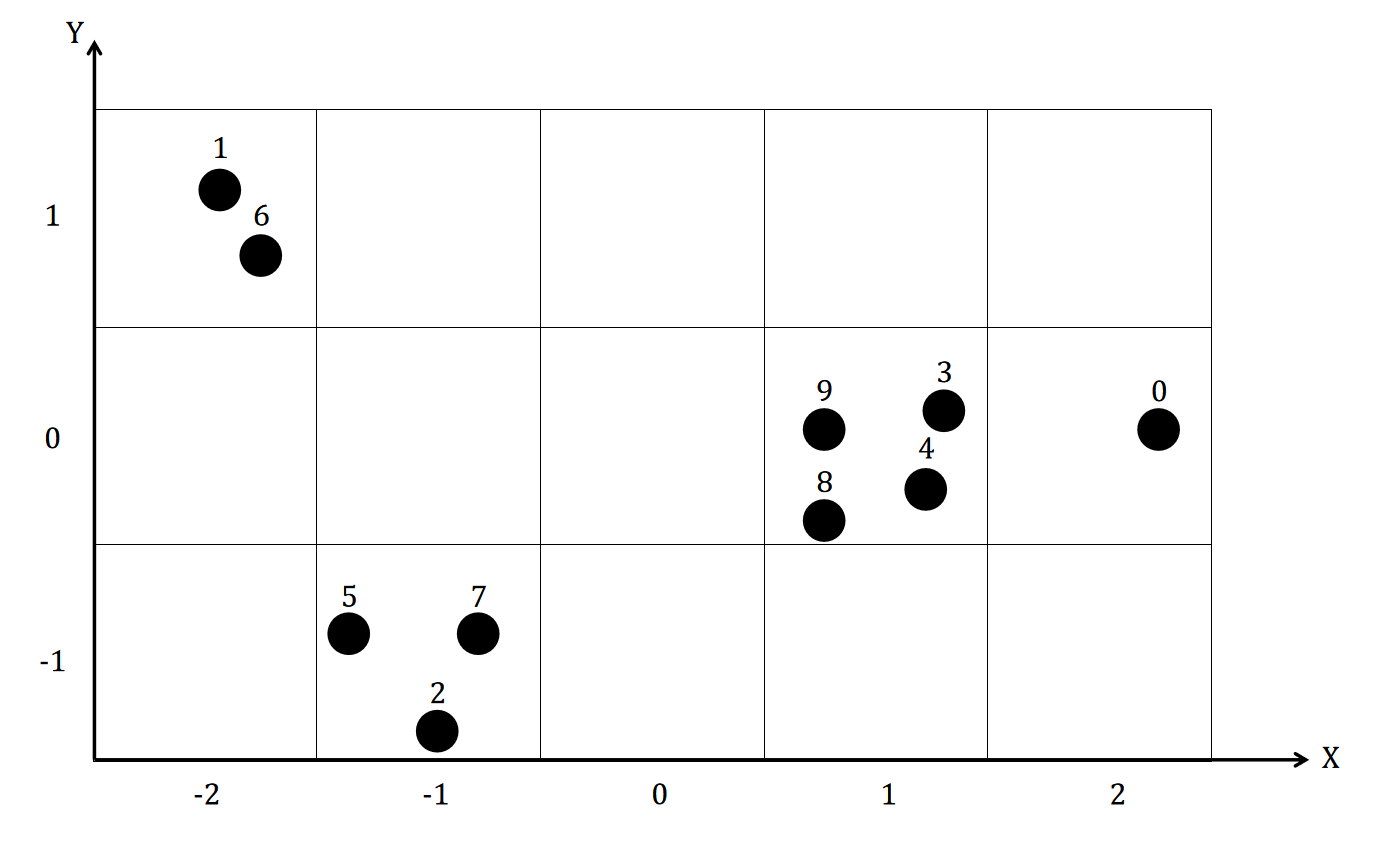
\includegraphics[height=5cm]{image/gridParticle.png}
    \bicaption{网格粒子分布示例}{Example of mesh particle distribution}
    \label{fig:gridParticle}
   \end{figure}


假设有十个粒子以如图所示的分布状态存在,当前只拥有每个粒子在世界空间坐标系下的位置,现在创建一个大小与粒子数目相同的数组,称为空间查找数组(Spatial Lookup)。对每个粒子计算其所在单元格的坐标。例如粒子0,位于单元格(2,0)。为了便于检索,我们需要将坐标转换为单个数字便于检索,可以通过将x和y坐标乘以两个不同的素数,然后相加,得到某个任意哈希值6613,再将它映射到数组长度上,变成了有效索引3,称为单元格键值,然后将单元格键值存储在空间查找数组下标为0处。接下来以此类推,遍历所有粒子,按照粒子在世界空间坐标系下的位置计算其所在单元格的位置,并将其对应的单元格键值存入空间查找数组中。
为了让在同一个单元格中的点在空间查找数组中彼此相邻从而有效地循环遍历它们。根据同一单元格的点具有相同的单元格键值,可以简单地根据这些键值对空间查找数组进行排序。得到如图从小到大排列单元格键值的数组,空间查找数组即初始化构建完成。其中所有位于同一单元格的粒子彼此相邻。
接下来我们创建同样与粒子数量等长的第二个数组,称为起始索引数组(Start Indices)。我们的最终目标是直接通过当前粒子邻域单元格的位置得到该单元格内所有粒子的索引。因此我们需要当得到某单元格位置时,存在一个数组,能够根据当前单元格位置对应的单元格键值查找空间查找数组中对应单元格键值的起始位置。因此需要起始索引数组,该数组在空间查找数组构建完成后扫描整个空间查找数组,记录所有连续相等的单元格键值的起始位置,并将其对应下标存在起始索引数组下标为当前单元格键值的位置。具体示例见图\ref{fig:gridArray}。
\begin{figure}[ht]
    \centering
    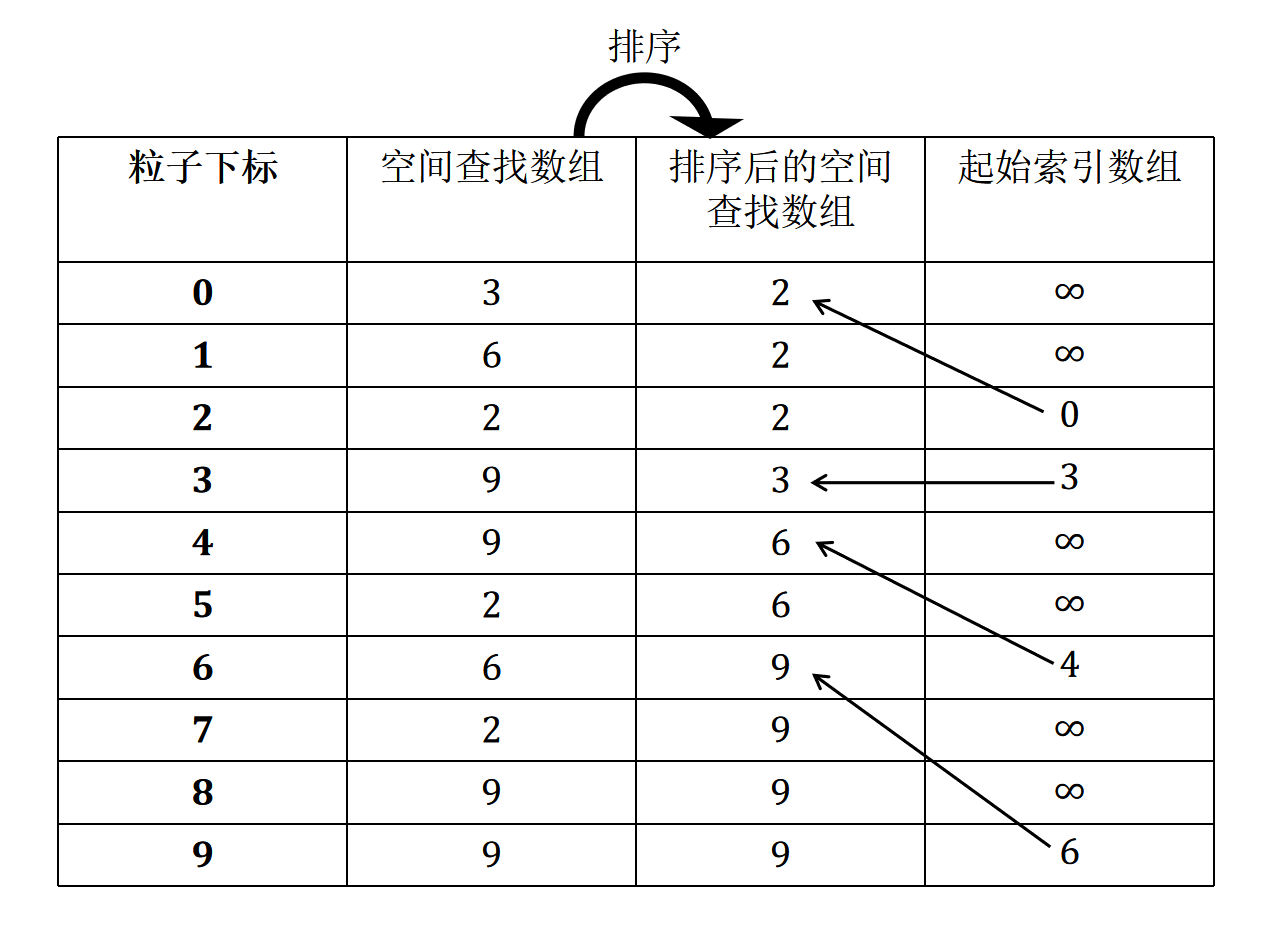
\includegraphics[height=5cm]{image/gridArray.png}
    \bicaption{空间查找数组和起始索引数组示意图}{Spatial lookup array and Start Indices array schematic}
    \label{fig:gridArray}
   \end{figure}
因为哈希函数自身的特点,会出现随机的单元格恰好和当前单元格有着相同的单元格键值。在进行遍历的时候,会对这个随机单元格中的额外粒子进行检查。这样的情况会造成一些时间上的消耗,而这种情况是在尝试实现具有无限内存的无限网格时所出现的结果。
在每次循环中需要重新构建一次空间查找数组和起始索引数组,但这两个数组为接下来求解密度、压力和粘度时提供了时间复杂度为$O(1)$的邻域查找速度。

% 计数排序
\subsubsection{并行排序算法优化}
在上述邻域搜索优化步骤中,对空间查找数组的排序是耗时最长的环节,因此有必要对排序算法进行优化。尽管在CPU上实现排序算法相对简单,而在GPU上排序由于GPU高度并行的单指令多数据(SIMD)架构而不太容易实现。但鉴于GPU在内存受限和计算受限算法方面的性能都优于CPU,因此找到在GPU上高效排序的方法非常重要。同时因为本文系统的目标是构建移动端实时流体仿真系统,因此优先考虑基于GPU的并行排序方法。
一个可选择的高效并行排序算法是双调归并排序算法。该算法的并行实现基本流程如图\ref{fig:bitonic}所示,每个工作线程对每对可排序元素做一次比较和交换操作,经互相独立的若干次交换之后就完成了整个数组的排序。这种并行方法的时间复杂度是$O(\log^2 n)$,并通过原地排序实现$O(1)$的空间复杂度,在排序时不消耗额外空间,且适用于任何数据结构。


\begin{figure}[ht]
    \centering
    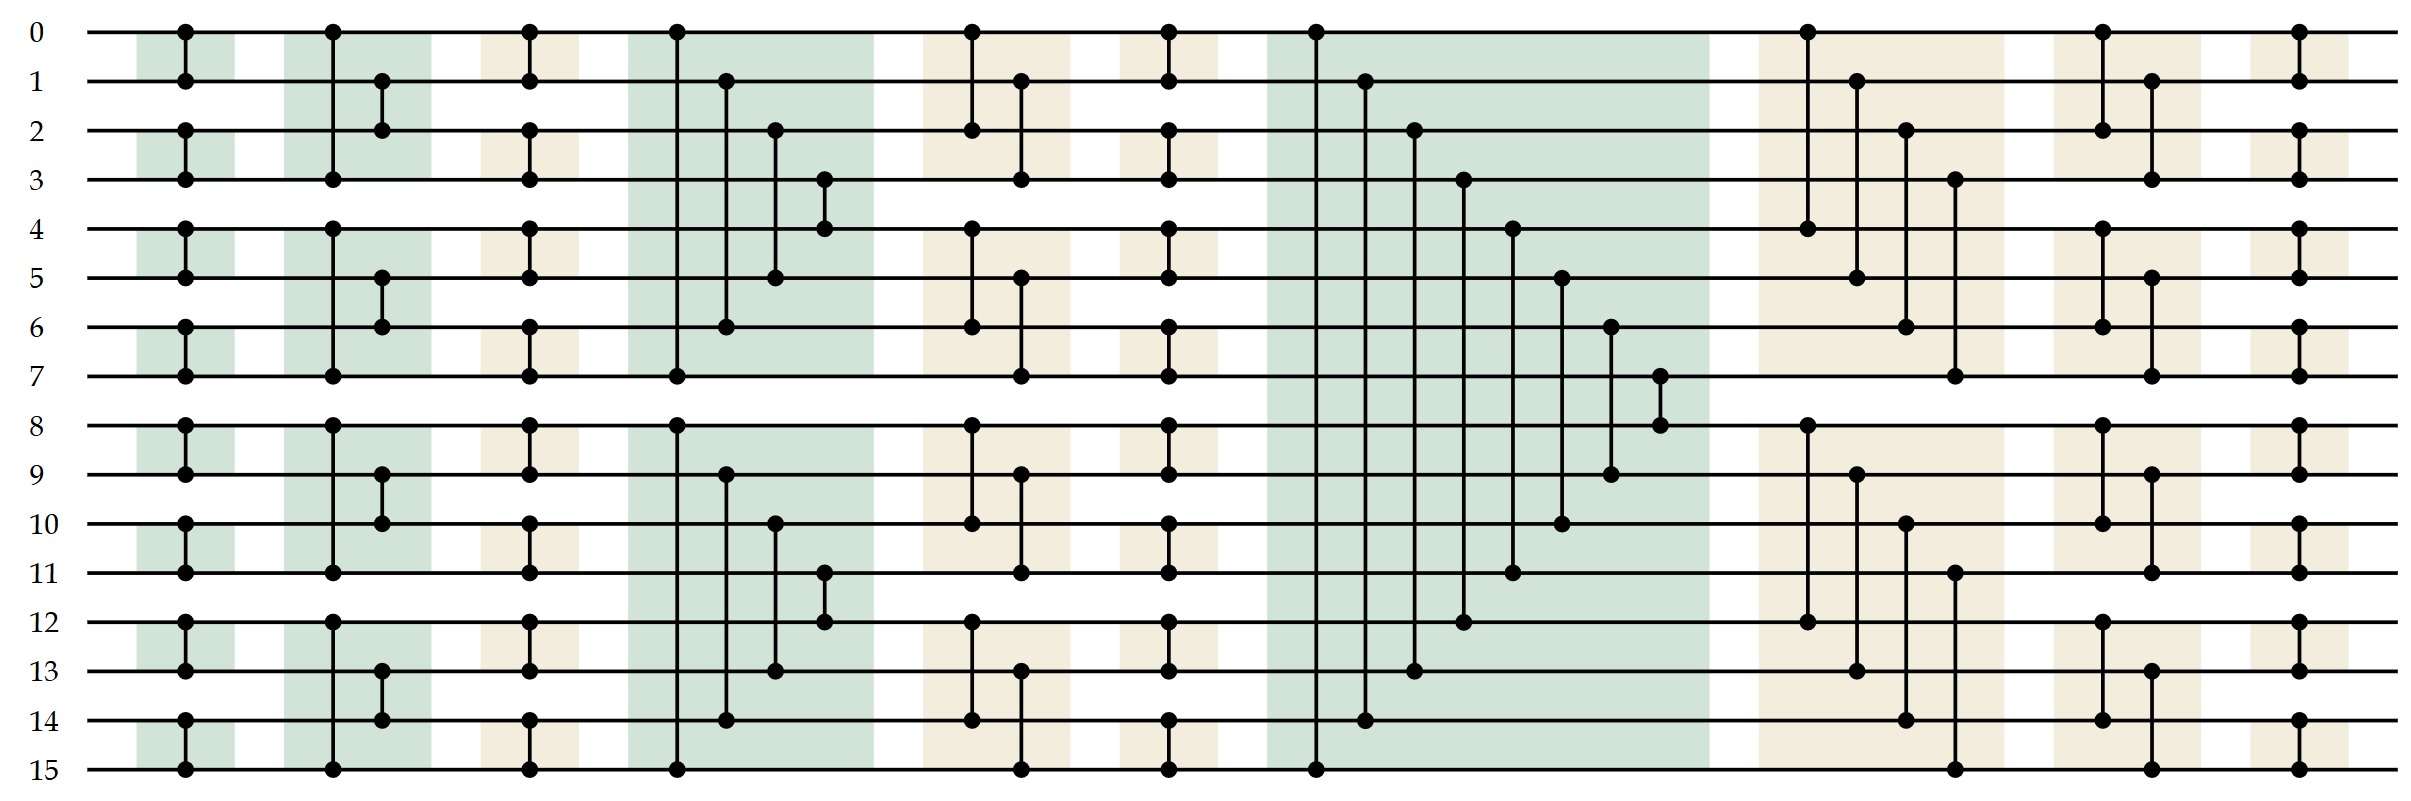
\includegraphics[height=5cm]{image/bitonicSort.png}
    \bicaption{双调归并排序算法示意图}{Schematic diagram of binary merge sorting algorithm}
    \label{fig:bitonic}
   \end{figure}

另一种并行排序算法是计数排序(Counting Sort)算法。计数排序是一种非比较排序算法,其核心思想是统计每个输入元素的个数,然后根据输入元素的大小,依次将其放入输出序列的正确位置。计数排序的时间复杂度为$O(n)$,空间复杂度为$O(n)$。计数排序只能对整数进行排序,且需要排序数据范围确定。
计数排序较双调排序更快,虽然需要更多空间,但在本文系统中,需要排序的数据范围不会超过粒子数目,因此在这种情况下,计数排序和双调排序消耗空间没有数量级上的差距。

基于上述分析,在本文系统中,我们采用计数排序(Counting Sort)算法。本文系统具体实现算法\ref{alg:countingSort}如下,首先进行初始化操作,创建一个长度为 maxValue + 1 的计数数组 Counts,并将所有元素设为 0,同时创建长度为 n 的排序后的数组 SortedItems 和 SortedKeys。接着计算每个键在原始数组 A 中的出现次数,并更新 Counts 数组。然后对 Counts 数组进行处理,计算每个键的前缀和。之后进行分散输出操作,从后向前遍历原始数组 A,根据 Counts 数组中的索引将元素放置在排序后的数组 SortedItems 和 SortedKeys 中,并同时更新 Counts 数组。最后将排序后的数组 SortedItems 和 SortedKeys 复制回输入数组 A 和 K,完成排序过程。

\begin{algorithm}
\caption{Counting Sort} \label{alg:countingSort}
\begin{algorithmic}[1]
\REQUIRE Array of items $A[1 \ldots n]$, Array of keys $K[1 \ldots n]$, Maximum key value $maxValue$
\ENSURE Sorted array $A$ and $K$

\STATE Initialize array $Counts[0 \ldots maxValue]$ to 0
\STATE Initialize array $SortedItems[1 \ldots n]$
\STATE Initialize array $SortedKeys[1 \ldots n]$

\FOR{each item $i$ in $A$}
    \STATE $Counts[K[i]] \leftarrow Counts[K[i]] + 1$
\ENDFOR

\FOR{each key $j$ from 1 to $maxValue$}
    \STATE $Counts[j] \leftarrow Counts[j] + Counts[j-1]$
\ENDFOR

\FOR{each item $i$ from $n$ down to 1}
    \STATE $SortedItems[Counts[K[i]]] \leftarrow A[i]$
    \STATE $SortedKeys[Counts[K[i]]] \leftarrow K[i]$
    \STATE $Counts[K[i]] \leftarrow Counts[K[i]] - 1$
\ENDFOR

\FOR{each item $i$ from 1 to $n$}
    \STATE $A[i] \leftarrow SortedItems[i]$
    \STATE $K[i] \leftarrow SortedKeys[i]$
\ENDFOR

\end{algorithmic}
\end{algorithm}




\section{移动端的参数优化}




\chapter{流体渲染方法}

\section{流体渲染的基本方法}
\section{渲染方法的性能分析}




\chapter{面向移动端的流体仿真系统}

\section{移动端流体仿真系统架构}
\section{流体仿真系统交互界面}



\chapter{实验与结果}

\section{渲染效果评估}
\section{仿真性能评估}


\chapter{结论}

\section{研究总结}
\section{贡献与展望}

